% !TeX encoding = UTF-8

\documentclass{protokol}

\usepackage{pdfpages}
\usepackage{tikz}
\usetikzlibrary{calc}
\usetikzlibrary{arrows}

%====== Units =====
\usepackage{siunitx}
\sisetup{inter-unit-product =\ensuremath{\cdot}}
\sisetup{group-digits = integer}
\sisetup{output-decimal-marker = {,}}
\sisetup{exponent-product = \ensuremath{\cdot}}
\sisetup{separate-uncertainty}
\sisetup{tight-spacing = false}
%\sisetup{scientific-notation = true}
%\sisetup{round-mode=places,round-precision=4}
%\sisetup{evaluate-expression}


%====== Grafy =====
\usepackage{pgfplots}
\pgfplotsset{width=0.8\linewidth, compat=1.17}
\def\plotcscale{0.8}
\usepackage{pgfplotstable}
\usepackage[figurename=Obr.]{caption} % figure caption rename

%====== Rovnice align block ======
\usepackage{amsmath}
\setlength{\jot}{10pt} % rozestup mezi řádky

\graphicspath{ {./img/} }

%====== Vyplňte údaje ======
\jmeno{Jakub Charvot}
\kod{240844}
\rocnik{3.}
\obor{MET}
\skupina{MET/2}
\spolupracoval{--}

\merenodne{19.02.\ 2024}
\odevzdanodne{25.02.\ 2024}
\nazev{Extrakce parametrů tranzistorů MOSFET ze SPICE modelu }
\cislo{1} %měřené úlohy

\predmet{Návrh analogových integrovaných obvodů}
\ustav{Ústav mikroelektroniky}
\skola{FEKT VUT v~Brně}

\def\para{x+0}
\def\parb{\para-80}


%citace 
\usepackage[backend=biber, style=iso-numeric, sortlocale=cs_CZ, autolang=other, language=czech]{biblatex}
\addbibresource{bibliography.bib}
\DeclareFieldFormat{labelnumberwidth}{\mkbibbrackets{#1}}
% hyperlinky
\usepackage[colorlinks]{hyperref}

% odstavce
\usepackage{parskip}

% Bloky kódu
\usepackage{xcolor}

%New colors defined below
\definecolor{codegreen}{rgb}{0,0.6,0}
\definecolor{codegray}{rgb}{0.5,0.5,0.5}
\definecolor{codepurple}{rgb}{0.58,0,0.82}
\definecolor{backcolour}{rgb}{0.95,0.95,0.92}

\usepackage{listings}
\lstdefinestyle{mystyle}{
  backgroundcolor=\color{backcolour}, commentstyle=\color{codegreen},
  keywordstyle=\color{magenta},
  numberstyle=\tiny\color{codegray},
  stringstyle=\color{codepurple},
  basicstyle=\ttfamily\footnotesize,
  breakatwhitespace=false,         
  breaklines=true,                 
  captionpos=b,                    
  keepspaces=true,                 
  numbers=left,                    
  numbersep=5pt,                  
  showspaces=false,                
  showstringspaces=false,
  showtabs=false,                  
  tabsize=2
}
\lstset{
	inputencoding=utf8,
	extendedchars=true,
	literate={á}{{\'a}}1 {č}{{\v{c}}}1 {ď}{{\v{d}}}1 {é}{{\'e}}1 {ě}{{\v{e}}}1 
           {í}{{\'i}}1 {ň}{{\v{n}}}1 {ó}{{\'o}}1 {ř}{{\v{r}}}1 {š}{{\v{s}}}1 
           {ť}{{\v{t}}}1 {ú}{{\'u}}1 {ů}{{\r{u}}}1 {ý}{{\'y}}1 {ž}{{\v{z}}}1 
           {Á}{{\'A}}1 {Č}{{\v{C}}}1 {Ď}{{\v{D}}}1 {É}{{\'E}}1 {Ě}{{\v{E}}}1 
           {Í}{{\'I}}1 {Ň}{{\v{N}}}1 {Ó}{{\'O}}1 {Ř}{{\v{R}}}1 {Š}{{\v{S}}}1 
           {Ť}{{\v{T}}}1 {Ú}{{\'U}}1 {Ů}{{\r{U}}}1 {Ý}{{\'Y}}1 {Ž}{{\v{Z}}}1,
	style=mystyle
	}

% Číslování
\pagenumbering{arabic}

% =========================================
% =============== DOKUMENT ================
% =========================================
\begin{document}
	%====== Vygenerování tabulky ======
	\maketitle

\section{Vypracování}
\begin{figure}[h!]
  \centering
  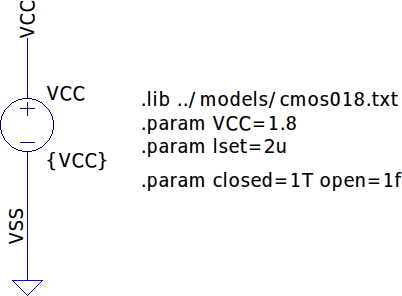
\includegraphics[scale=0.5]{spice0.png}
  \caption{Společná část SPICE kódu a napájecí zdroj.}
  \label{fig:spice0-png}
\end{figure}
 
\subsection{Zdroj referenčního proudu}
  \begin{figure}[h!]
    \centering
    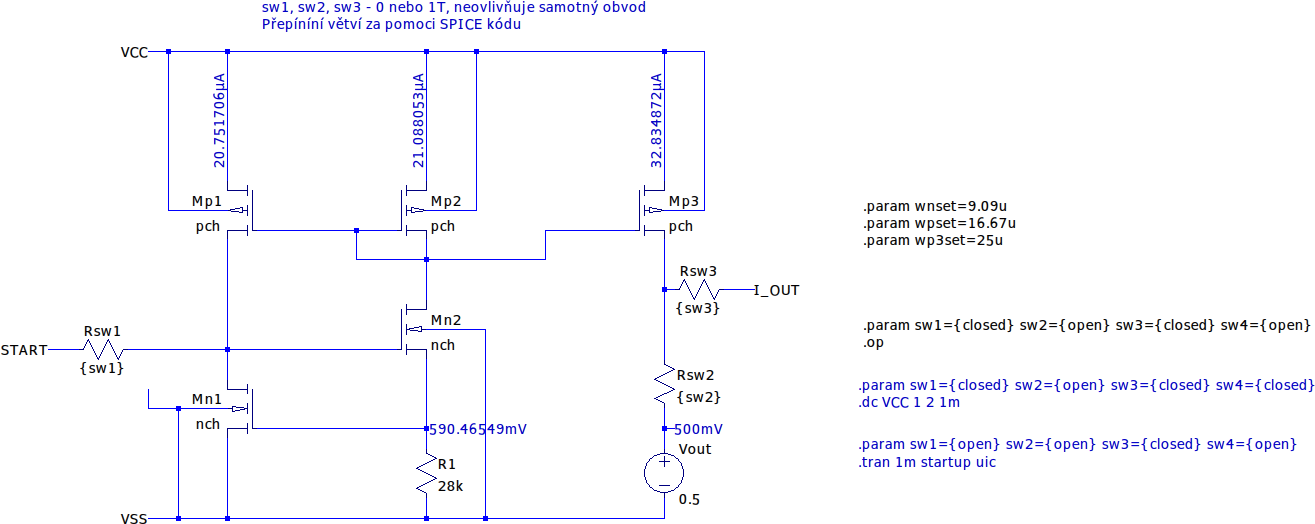
\includegraphics[scale=0.5]{spice2.png}
    \caption{Proudová reference, analýza OP.}
    \label{fig:spice0-png}
  \end{figure}

  \begin{figure}[h!]
    \centering
    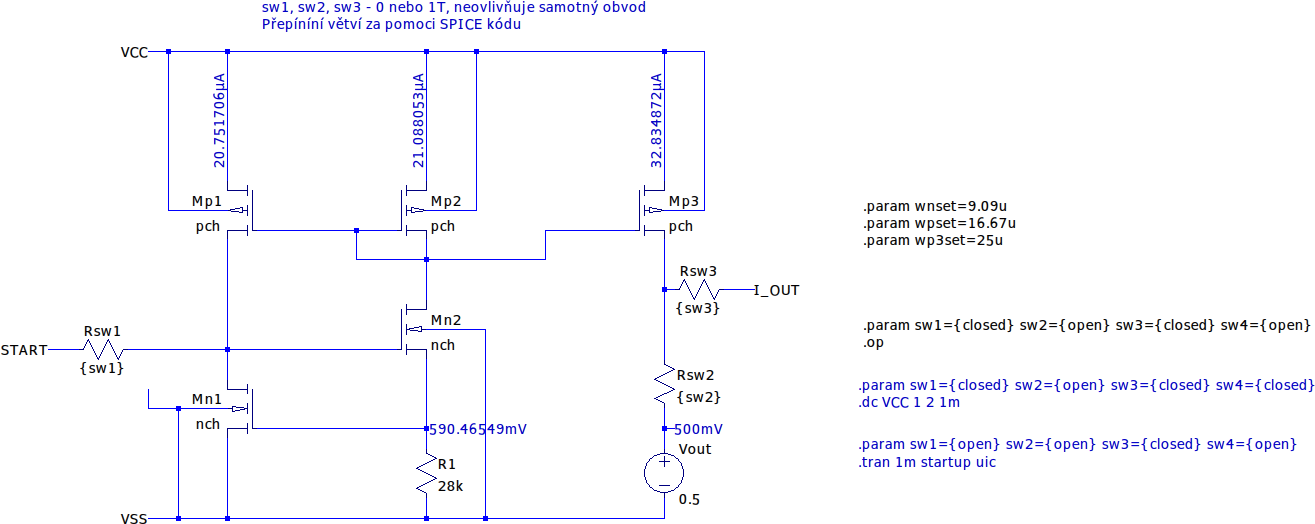
\includegraphics[scale=0.5]{spice2.png}
    \caption{Proudová reference, analýza OP -- C2 vnutí prac. bod.}
    \label{fig:spice0-png}
  \end{figure}

  \begin{figure}[h!]
    \centering
    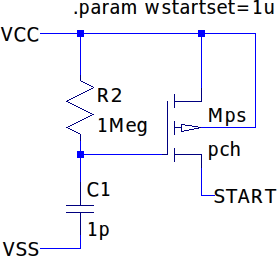
\includegraphics[scale=0.5]{spice1.png}
    \caption{Startovací obvod.}
    \label{fig:spice0-png}
  \end{figure}


\clearpage
\subsubsection{Ruční návrh}
Nejprve vypočítám rozměry pro tranzistor \(M_{N1} \):
\[
    \frac{W_{N1} }{L}=\frac{2\cdot I_{D}}{KP_{N}\cdot (U_{GS} -U_{TH})^2 } 
\]
\[
    \frac{W_{N1} }{L}=\frac{2\cdot \num{20e-6}}{\num{220e-6}\cdot (\num{0.2})^2 } 
\]

\[
    \frac{W_{N1} }{L}\doteq \num[round-mode=places,round-precision=2]{4.545454545454545} 
\]
Délku \(L\) zvolíme opět \qty{2}{\micro\meter}, tedy \(W_{N1}= \qty{9.09}{\micro\meter}\). Pro tranzistor \(M_{N2} \) zvolíme stejné rozměry.

Pro tranzistory \(M_{P1} \) a \(M_{P2} \) vypočteme rozměry obdobným způsobem:

\[
    \frac{W_{P12} }{L}=\frac{2\cdot I_{D}}{KP_{P}\cdot (U_{GS} -U_{TH})^2 } 
\]
\[
    \frac{W_{P12} }{L}=\frac{2\cdot \num{20e-6}}{\num{60e-6}\cdot (\num{0.2})^2 } 
\]

\[
    \frac{W_{P12} }{L}\doteq \num[round-mode=places,round-precision=2]{16.666666666666664}
\]

Pro stejnou délku \(L\) pak vychází \(W_{P12}=\qty{33.33}{\micro\meter} \).

Dále je potřeba stanovit hodnotu odporu \(R_{1} \), úbytek napětí na něm odpovídá napětí napětí \(U_{GS} \) pro tranzistor \(M_{N1} \):
\begin{align*}
    R_{1} =& \frac{U_{R1}}{I_{R1}} \\
          =& \frac{U_{GS,M1}}{I_{M,N2}} \\
          =& \frac{U_{TH0,N1}+U_{OV,N1} }{I_{M,N2}} \\
          =& \frac{\num{360e-3}+\num{0.2} }{\num{20e-6}} \\
          =& \qty{28}{\kilo\ohm}
\end{align*}

Pro výstupní větev je požadován jiný proud, upravíme tedy rozměry tranzistoru \(M_{P3} \):
\begin{align*}
    W_{P3} =& \frac{3}{2}\cdot W_{P2} \\
           =& \frac{3}{2}\cdot \num{16.67} \\
           =& \qty{25}{\micro\meter}
\end{align*}

Výstupní odpor zapojení je dán tranzistorem \(M_{P3} \):
\[
    r_{OUT} = \frac{1}{\lambda I_{MP3} }=\frac{1}{\num{0.08}\cdot \num{30e-6}}=\qty{416.67}{\kilo\ohm}
\]

\subsubsection{Simulace}

\begin{figure}[h!]
    \centering
    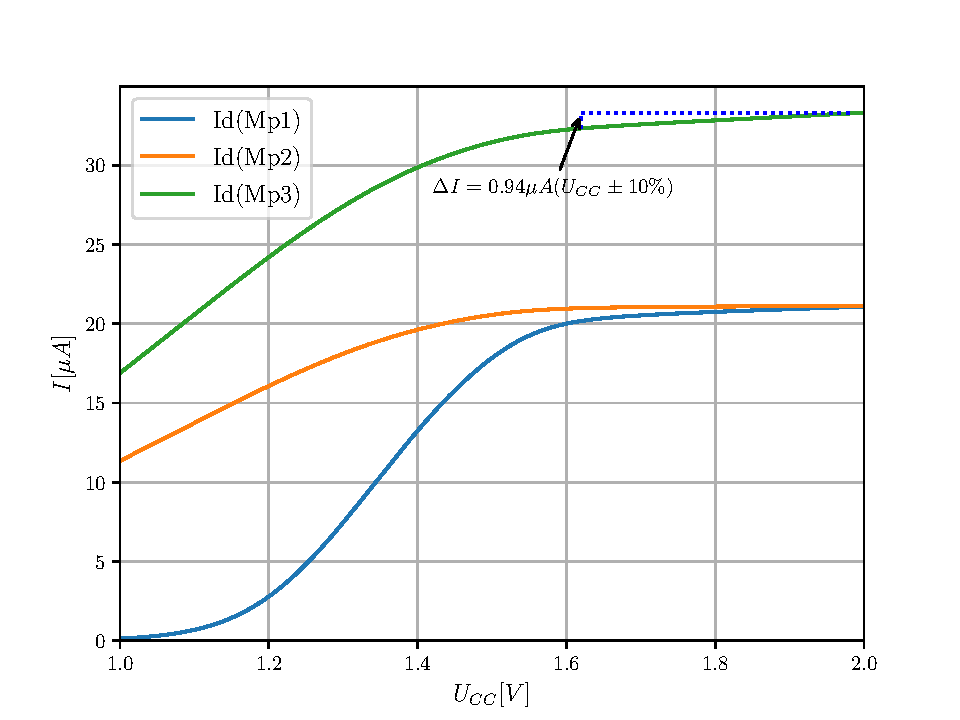
\includegraphics[width=0.8\textwidth]{img/3-1-4.pdf}
    \caption{Závislost proudů v obvodu na změně napájecího napětí.}
    \label{fig:img/3-1-4.pdf}
\end{figure}


\begin{figure}[h!]
    \centering
    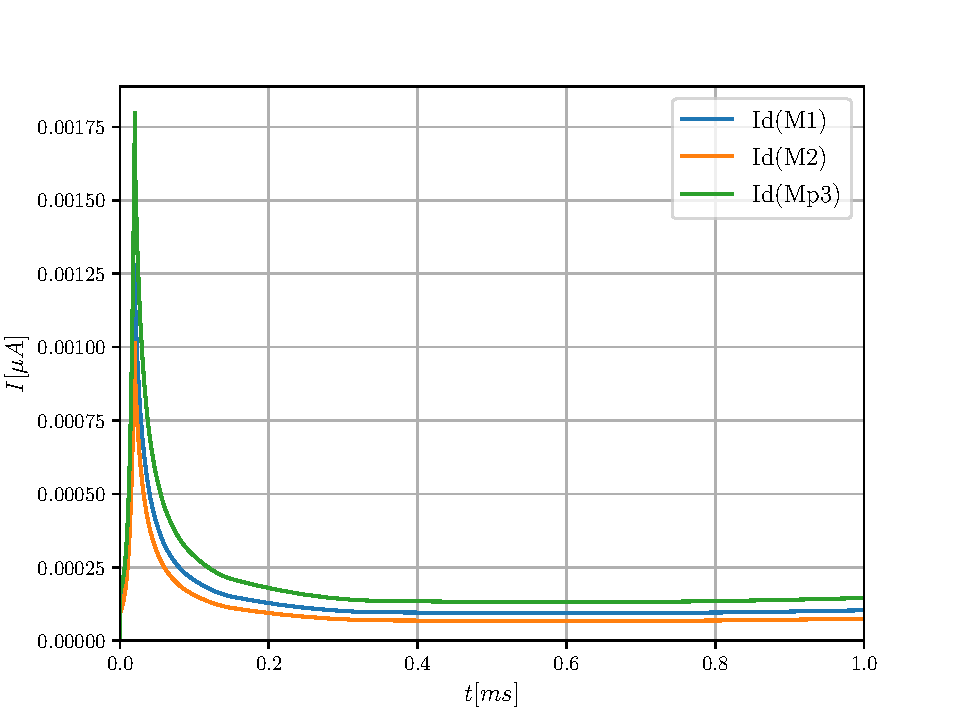
\includegraphics[width=0.8\textwidth]{img/3-1-5.pdf}
    \caption{Časová analýza zapojení bez startovacího obvodu (sw1=closed).}
    \label{fig:img/3-1-5.pdf}
\end{figure}

\begin{figure}[h!]
    \centering
    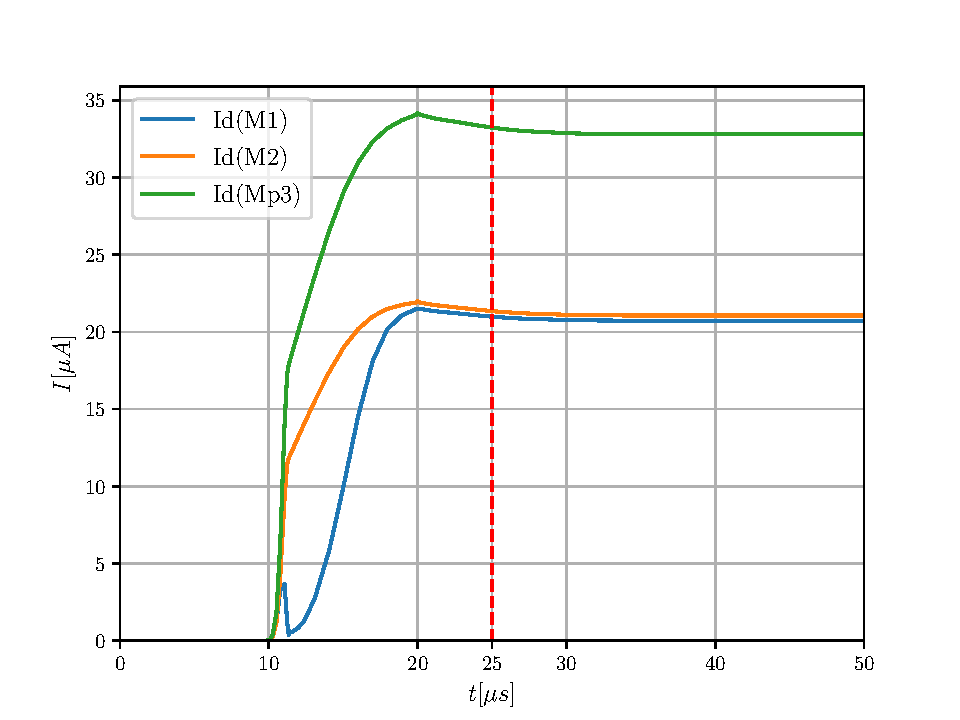
\includegraphics[width=0.8\textwidth]{img/3-1-6.pdf}
    \caption{Časová analýza zapojení se startovacím obvodem (sw1=open).}
    \label{fig:img/3-1-6.pdf}
\end{figure}


  \clearpage
\subsection{Zdroj referenčního napětí }
\begin{figure}[h!]
    \centering
    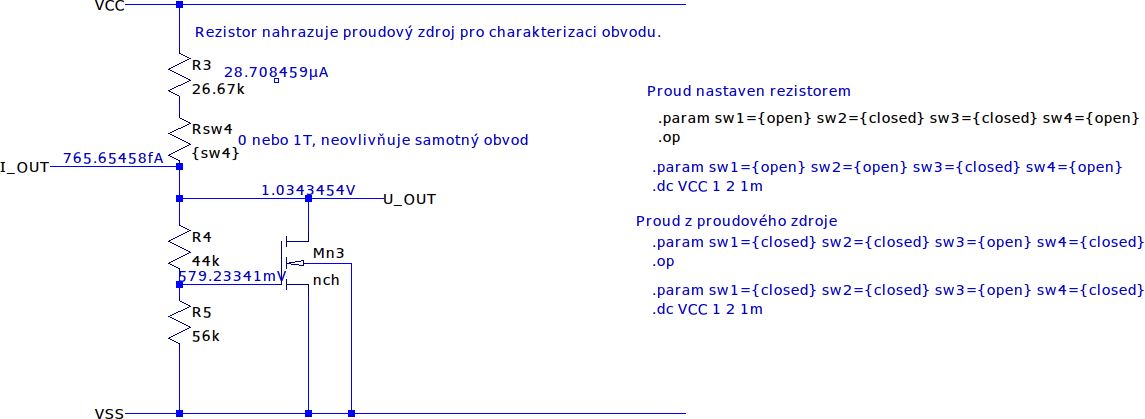
\includegraphics[scale=0.5]{spice2-1.png}
    \caption{Napěťová reference, analýza OP -- proud přes rezistor.}
    \label{fig:spice0-png}
  \end{figure}

  \begin{figure}[h!]
    \centering
    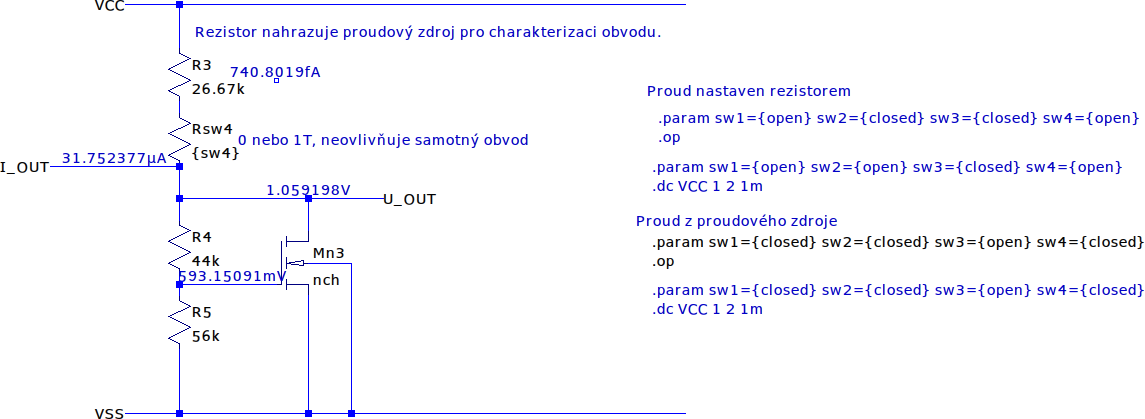
\includegraphics[scale=0.5]{spice2-2.png}
    \caption{Napěťová reference, analýza OP -- proud z proud. reference.}
    \label{fig:spice0-png}
  \end{figure}


\clearpage
\subsubsection{Ruční návrh}
Proud z proudového zdroje se rozdělí do dvou větví, tranzistorem necháme procházet větší část, konkrétně \qty{20}{\micro\ampere}, pro jeho rozměry pak platí:
Nejprve vypočítám rozměry pro tranzistor \(M_{N3} \):
\[
    \frac{W_{N3} }{L}=\frac{2\cdot I_{D}}{KP_{N}\cdot (U_{GS} -U_{TH})^2 } 
\]
\[
    \frac{W_{N3} }{L}=\frac{2\cdot \num{20e-6}}{\num{220e-6}\cdot (\num{0.2})^2 } 
\]

\[
    \frac{W_{N3} }{L}\doteq \num[round-mode=places,round-precision=2]{4.545454545454545} 
\]
Délku \(L\) zvolíme opět \qty{2}{\micro\meter}, tedy \(W_{N3}= \qty{9.09}{\micro\meter}\). 

Odporovou větví tedy prochází proud \(I_{R} =\qty{10}{\micro\ampere}\), který na rezistoru \(R_{5} \) tvoří úbytek napětí rovný napětí \(U_{GS} \) tranzistoru. Pro hodnoty rezitorů platí:
\begin{align*}
    R_{5} =& \frac{U_{R5}}{I_{R}} \\
          =& \frac{U_{GS,MN3}}{I_{R}} \\
          =& \frac{U_{TH0,N3}+U_{OV,N3} }{I_{R}} \\
          =& \frac{\num{360e-3}+\num{0.2} }{\num{10e-6}} \\
          =& \qty{56}{\kilo\ohm}
\end{align*}
\begin{align*}
    R_{4} =& \frac{U_{REF}}{I_{R}} - R_{1}  \\
          =& \frac{1}{\num{10e-6}} - \num{56e3}  \\
          =& \qty{44}{\kilo\ohm}
\end{align*}
Pro nastavení proudu použjeme rezistor \(R_{3} \):
\begin{align*}
    R_{3} =& \frac{U_{CC} - U_{REF}}{\num{30e-6}}  \\
          =& \frac{\num{1.8} - 1}{\num{30e-6}}  \\
          =& \qty{26.67}{\kilo\ohm}
\end{align*}




\subsubsection{Simulace}

\begin{figure}[h!]
    \centering
    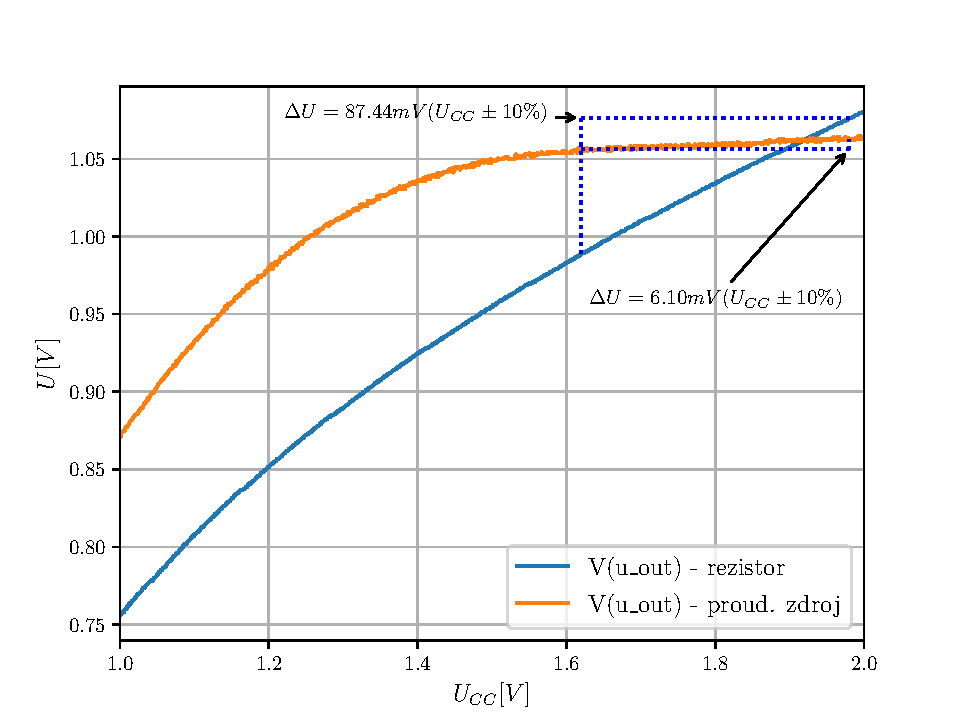
\includegraphics[width=0.8\textwidth]{img/3-2-3.pdf}
    \caption{Časová analýza -- srovnání výstupů napěťové reference.}
    \label{fig:img/3-2-3.pdf}
\end{figure}

\clearpage
\section{Závěr}
  V první části úlohy šlo o vytvoření proudové reference nezávislé na napájecím napětí, na Obr. \ref{fig:img/3-1-4.pdf} lze vidět, že zcela nezávislá není, ale výstupní proud je podstatně stabilnější než v předchozí úloze. 

  Abychom spolehlivě zajistili dosažení správného pracovního bodu, je potřeba připojit tzv. startovací obvod, pro zvolené hodnoty součástek dojde k dosažení prac. bodu v čase přibližně \qty{25}{\micro\second} po připojení napájení (viz Obr. \ref{fig:img/3-1-6.pdf}). 

  Ve druhé části úlohy jsme vytvářeli jednoduchou napěťovou referenci, ta ke své funkci potřebuje proudový zdroj. Nakolik bude napěťová reference nezávislá na změně napájecího napětí záleží zejména na kvalitě použitého proudového zdroje. Jenoduchý rezistor není příliš vhodný (z hlediska nezávislosti výstupu) a je vhodné jako vstup využít např. námi vytvořenou proudovou referenci. Porovnání obou scénářů se nachází na Obr. \ref{fig:img/3-2-3.pdf}. 

  Co se týče mého způsobu "spínání" částí obvodu za pomoci rezistorů s malou resp. velkou hodnotou odporu, která principiálně neovlivní dané zapojení, nemohu říci, že by se metoda osvědčila. V několika simulacích jsem musel od tohoto způsobu upustit, protože SPICE se zřejmě pro některé uzly dostával k hodnotám příliš malým a pracoval velmi neefektivně nebo simulace nekonvergovala vůbec, pro příště tedy budu muset zvolit jiný způsob.  

% \section*{Reference}
% \printbibliography[heading=none]


\end{document}